%\documentclass[aps,prb,amsmath,twocolumn,amssymb,titlepage]{revtex4-1}
\documentclass[10pt]{revtex4-1}
\usepackage{graphicx}
\usepackage{nicefrac}
\usepackage{amsfonts}
\usepackage{amssymb}
\usepackage{amsmath} 
\usepackage{subfigure}
\usepackage{multirow} 
\usepackage{tabularx} 
\usepackage{array}
\usepackage{units}
\usepackage{tensor} 
\usepackage{braket}
\usepackage{bm}
\usepackage{hyperref}
\usepackage[resetlabels, labeled]{multibib}
%\newcites{supp}{References}

\renewcommand{\Re}{\operatorname{{\mathrm Re}}}
\renewcommand{\Im}{\operatorname{{\mathrm Im}}}
\newcommand{\tr}{\operatorname{{\mathrm tr}}} 

\newcommand{\hc}{^{\dagger}}
\newcommand{\ad}{\operatorname{{\mathrm ad}}}
\newcommand{\adn}{\ad_{\hat n}}
\newcommand{\adx}{\ad_{\hat x}}
\newcommand{\adX}[1][]{\ad_{\hat {\mathbf{X}}_{#1}}}
\newcommand{\adp}{\ad_{\hat p}}
\newcommand{\calD}{\mathcal{D}}    %Caligraphic D
\newcommand{\inbk}[1]{\left[ #1 \right]}
\newcommand{\inbr}[1]{\left\{ #1 \right\}}
\newcommand{\inp}[1]{\left( #1 \right)}
\newcommand{\pd}{\partial}
\newcommand{\pdf}[3]{\frac{\pd^{#1} #2}{\pd #3^{#1}}} %Partial derivative
\newcommand{\fdf}[3][]{\frac{\delta^{#1} #2}{\delta #3^{#1}}} %Functional
                                %derivative 

\newcommand\xSOne{$X_{\mathcal{S}_1}$}
\newcommand\xcSEOne{$\hat{X}^c_{\mathcal{S}_1,\mathcal{E}_1}$}
\newcommand\xsSOOne{$\hat{X}^s_{\mathcal{S}_1,\mathcal{O}_1}$}
\newcommand\xSTwo{$X_{\mathcal{S}_2}$}
\newcommand\xcSETwo{$\hat{X}^c_{\mathcal{S}_2,\mathcal{E}_2}$}
\newcommand\xsSOTwo{$\hat{X}^s_{\mathcal{S}_2,\mathcal{O}_2}$}

\begin{document}
\nocite{*}

\begin{figure}
  \centering
  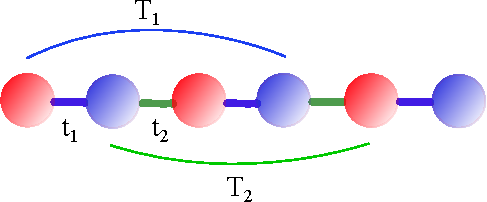
\includegraphics[width=.37\textwidth]{./phase_diagrams/ssh_model.pdf}
  \caption{Schematic set-up of a 1D SSH system. Here $t_1$ and $t_2$ are nearest-neighbor hoppings while $T_1$ and $T_2$ are second nearest-neighbor hoppings.}
\label{fig:model}
\end{figure}

\begin{figure}%[h!]
  \centering
  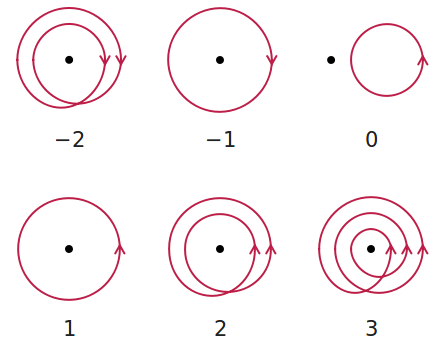
\includegraphics[width=.37\textwidth]{./phase_diagrams/winding.png}
  \caption{Winding number. The winding number of a closed, oriented curve with respect to a reference point is a topological invariant that counts how many times the curve winds around the point. Picture credits: Jim Belk, public domain.}
\label{fig:winding}
\end{figure}

\section*{Supplementary Material}
\subsection*{The SSH model}
\label{sshapp}

The SSH model \cite{asboth2016short} describes the movement of free electrons along a dimerized chain whose basic units consist of two distinct atoms. This movement, usually called ``hopping'' in the literature, can be made either between atoms in a unit cell or between unit cells, and the allowed hopping rules for a given system completely determine its Hamiltonian. This is because the kinetic energies of the electrons are parameterized by a vector of real numbers $\mathbf{t}$ that also encodes hopping terms, thus allowing for a compact mathematical description of a Hamiltonian in terms of creation/annihilation operators as
\begin{equation}
\label{SSH}
\mathbf{H}(\mathbf{t})=\mathbf{c}^{\dagger}H(\mathbf{t})\mathbf{c}
\end{equation}
where the column vector
\begin{equation*}
\mathbf{c} =\Big(c^{A}_1,c^{B}_1,\cdots,c^{A}_\frac{N}{2},c^{B}_\frac{N}{2}\Big)^T
\end{equation*}
contains annihilation operators $c^{A(B)}_p$ that erase electrons at atom A (B) and lattice site $p$ and similarly the row vector
\begin{equation*}
\mathbf{c}^\dagger =\Big(c^{A\dagger}_1,c^{B\dagger}_1,\cdots,c^{A\dagger}_\frac{N}{2},c^{B\dagger}_\frac{N}{2}\Big)
\end{equation*}
contains creation operators $c^{A(B)\dagger}_p$ that produce electrons at atom A (B) and lattice site $p$. Please note that $N$ is twice the number of unit cells in the chain and therefore an even integer.

The convenience of equation \eqref{SSH} is that all information about a system such as its eigenstates and eigenenergies can be recovered from the $N\times N$ matrix $H(\mathbf{t})$. We can thus think of the vectors $\mathbf{t}$ in parameter space as very compact representations of SSH models: each point in $\mathbf{t}$-space can be mapped to a $N\times N$ matrix $H(\mathbf{t})$ whose eigenvectors and eigenvalues can then be computed, as is usually done in quantum mechanics. As an example, a general matrix $H(\mathbf{t})$ describing a SSH system with hoppings between nearest and second nearest neighbors is given by
\begin{equation}\label{hmatrix}
H(t_1,t_2,T_1,T_2)=\left(
  \begin{array}{cccccc}
    0 & t_1 & 0 & T_1 & 0 & \cdots \\
    t_1 & 0 & t_2& 0 & T_2 & \cdots\\
    0 & t_2 & 0 & t_1 & 0 & \cdots\\
    T_1 & 0 & t_1 & 0 & t_2 & \cdots\\
    0 & T_2 & 0 & t_2 &  0& \cdots\\
    \vdots & \vdots    & \vdots & \vdots &  \vdots & \ddots\\
  \end{array}
  \right)_{N \times N}.
\end{equation}
Knowing the vector $\mathbf{t}=(t_1,t_2,T_1,T_2)$ corresponding to a particular system described by the Hamiltonian in equation \eqref{hmatrix} should suffice to compute any of its physical properties, including its topological phase. Figure \ref{fig:model} depicts a SSH system described by equation \eqref{hmatrix}.

The reason why topological materials garnered so much interest in recent years is that their physical properties are topologically robust.
This means that these properties are stable under continuous (i.e., adiabatic) mathematical operations performed on the system's underlying wave functions. This topological robustness is expressed theoretically in terms of a topological invariant that characterizes different phases of a system. In the particular case of the SSH model, the topological invariant used to classify the topological phases is the winding number.

The winding number is a topological property of any closed, oriented curve that measures how many times the curve winds around a point that does not belong to itself. It can be any integer and is usually chosen to be positive when the curve winds in counterclockwise motion with respect to the reference point (equivalently, when a closed, oriented curve winds in clockwise motion around a reference point its winding number is negative). Figure \ref{fig:winding} shows several closed, oriented curves and their winding numbers computed with respect to a given point.

An interesting property of topological invariants like the winding number is that they are a global feature of geometric objects: for each of the curves in figure \ref{fig:winding} for example the winding number is a property of the whole curve that cannot be defined locally for each of its points. This fundamental characteristic of topological invariants makes the study of topological phases of matter from local lattice data a challenging task.   

For SSH systems with translational symmetry like the finite systems with periodic boundary conditions investigated in the article, the winding number is usually computed in wavevector space via
\begin{equation}\label{winding_number}
W=\frac{1}{4\pi i}\int_0^{2\pi} dk Tr( \sigma_3 H(k)^{-1} \partial_k H(k)),
\end{equation}
where $H(k)$ is the kernel in wavevector space of a Hamiltonian $\mathbf{H}$$($$\mathbf{t}$$)$ and $\sigma_3$ is the chiral operator. Equation \eqref{winding_number} can be evaluated for several Hamiltonians by varying the parameter $\mathbf{t}$, resulting in phase diagrams in parameter space like the ones shown in figure 1 in the article. %\ref{fig:phasediagrams}.

\begin{figure}
\centering
\subfigure[]{\label{eng_feat_ssh1:a}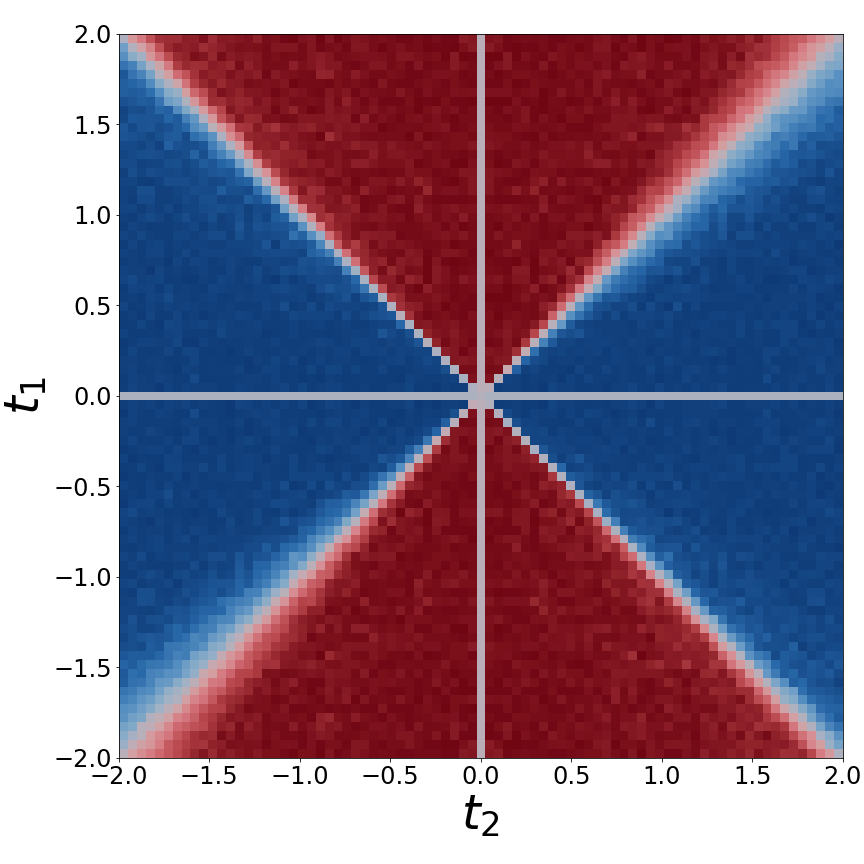
\includegraphics[width=.32\textwidth]{./supp_figures/ssh1/periodic_100_6561/real_space_best_04_sites/merge_imshow_winding_grids_second_sim.png}}
\subfigure[]{\label{eng_feat_ssh1:b}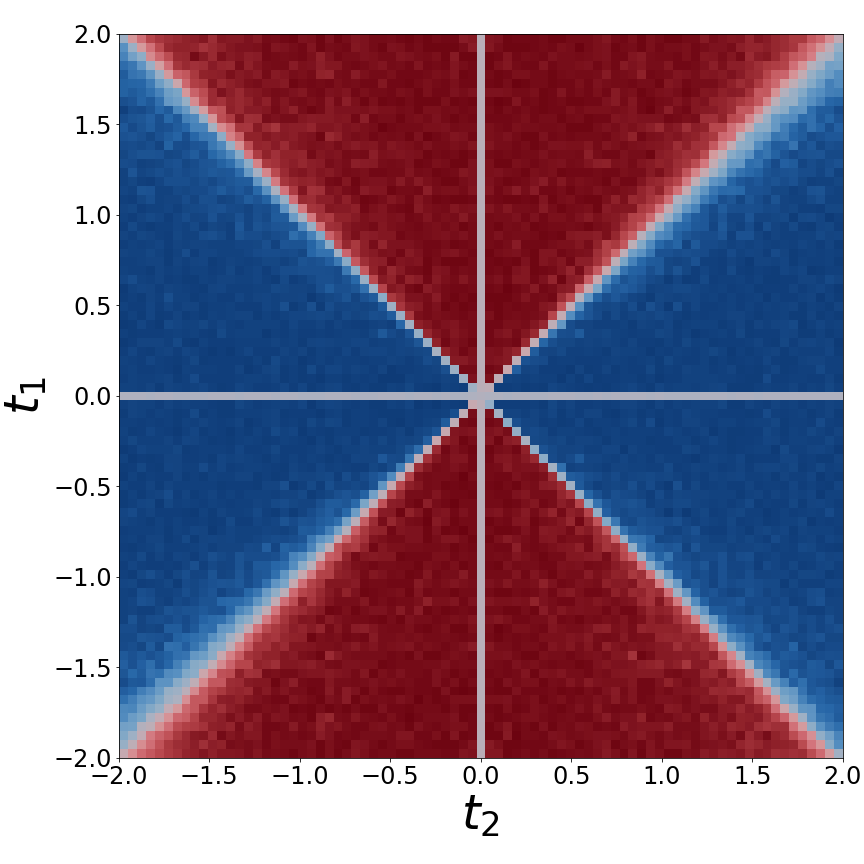
\includegraphics[width=.32\textwidth]{./supp_figures/ssh1/periodic_100_6561/dct_best_04_wavevector_sites_from_best_04_real_space_sites/merge_imshow_winding_grids_second_sim.png}}
\subfigure[]{\label{eng_feat_ssh1:c}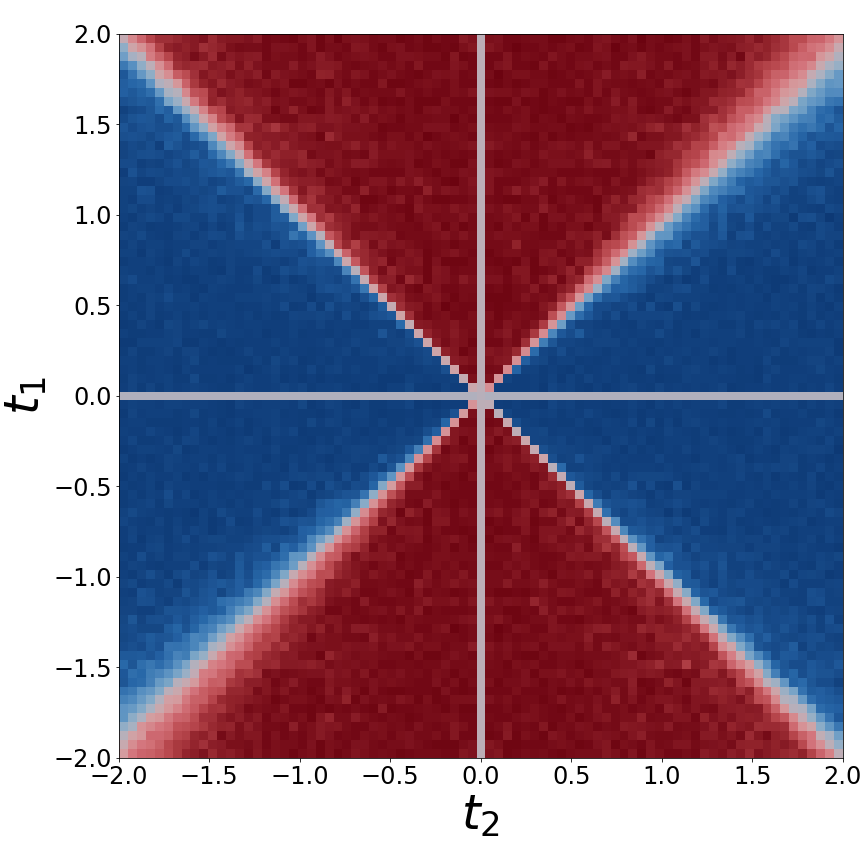
\includegraphics[width=.32\textwidth]{./supp_figures/ssh1/periodic_100_6561/dst_best_04_wavevector_sites_from_best_04_real_space_sites/merge_imshow_winding_grids_second_sim.png}}
\caption{Phase diagrams learned from compressed representations of the SSH 1 system. (a) Phase diagram learned using the real space features \xSOne.  (b) Phase diagram learned from the DCT topological features \xcSEOne. (b) Phase diagram learned from the DST topological features \xsSOOne.}
\label{eng_feat_ssh1}
\end{figure}

\begin{figure}
\centering
\subfigure[]{\label{eng_feat_ssh2:a}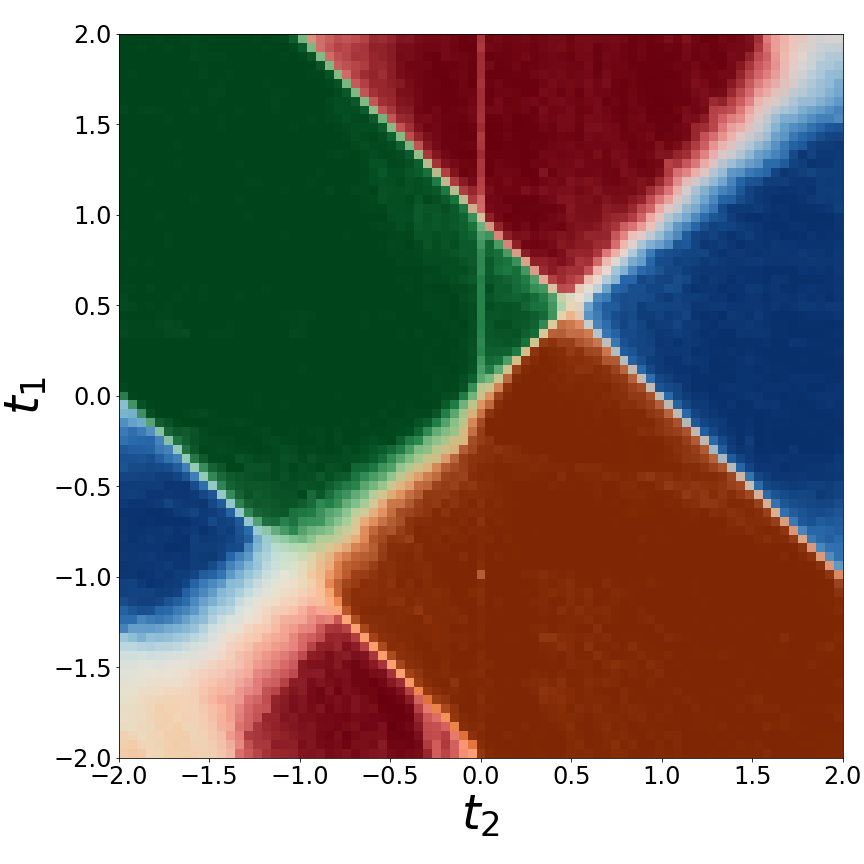
\includegraphics[width=.32\textwidth]{./supp_figures/ssh2/periodic_100_6561/real_space_best_12_sites/merge_imshow_winding_grids_sim.png}}
\subfigure[]{\label{eng_feat_ssh2:b}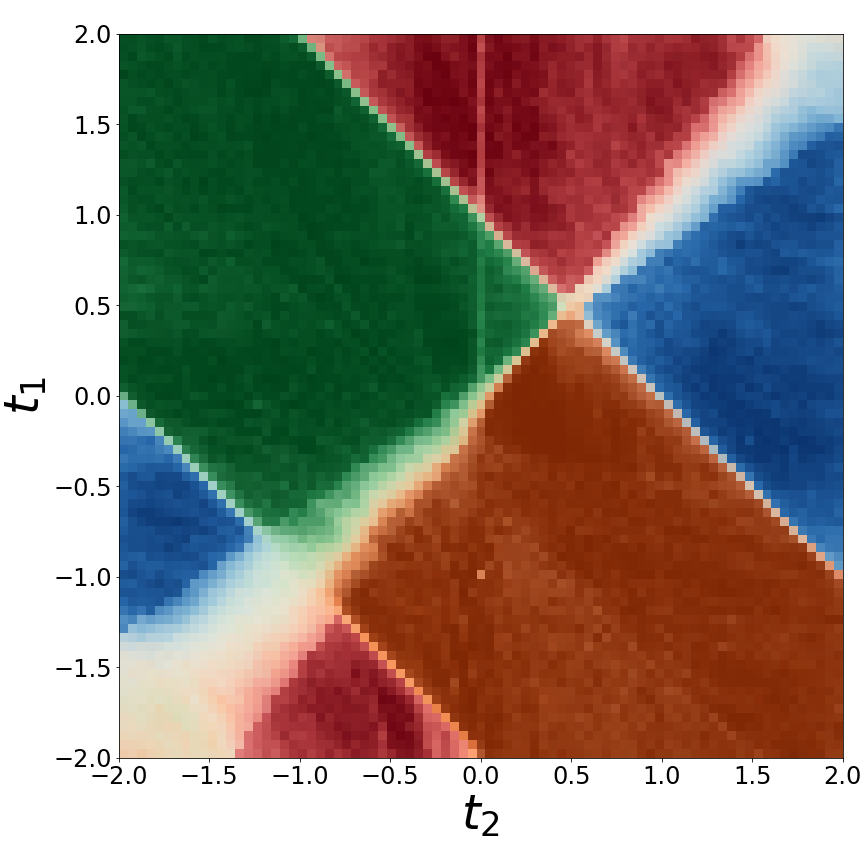
\includegraphics[width=.32\textwidth]{./supp_figures/ssh2/periodic_100_6561/dct_best_12_wavevector_sites_from_best_12_real_space_sites/merge_imshow_winding_grids_sim.png}}
\subfigure[]{\label{eng_feat_ssh2:c}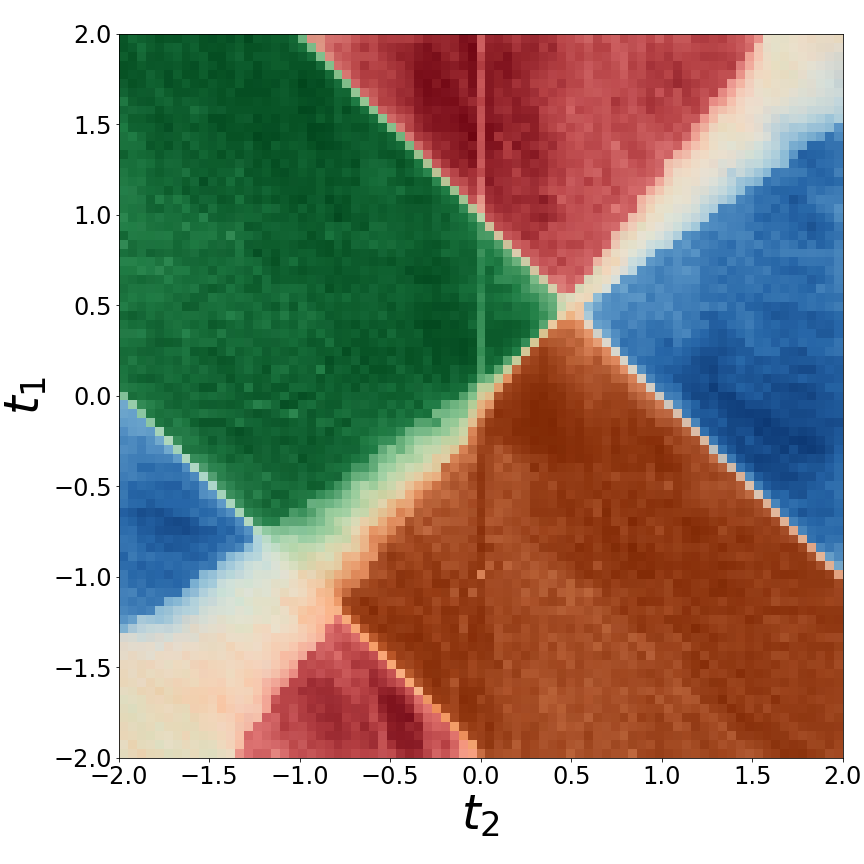
\includegraphics[width=.32\textwidth]{./supp_figures/ssh2/periodic_100_6561/dst_best_12_wavevector_sites_from_best_12_real_space_sites/merge_imshow_winding_grids_sim.png}}
\caption{Phase diagrams learned from compressed representations of the SSH 2 system. (a) Phase diagram learned using the real space features \xSTwo.  (b) Phase diagram learned from the DCT topological features \xcSETwo. (b) Phase diagram learned from the DST topological features \xsSOTwo.}
\end{figure}

\subsection*{Learning topological phases from real space data}

%The main motivations for developing a data-driven approach based on real space are that wavevector space computations such as eq. %\eqref{winding_number} are only possible for systems with translational symmetry, which many physical systems of current interest (e.g. %disordered systems in condensed matter) do not have. Moreover, since real space and wavevector space eigenvectors are related by Fourier %transforms, the latter are essentially delocalized and therefore so is any information recovered from them. We argue here that a data-driven %approach based on real space offers a viable alternative to wavevector space computations that addresses these shortcomings.

The insights behind our intuition that topological phases can be learned from local features are as follows. First, while the topological invariants that characterize distinct topological phases are usually computed in wavevector space, the topological properties of a Hamiltonian are the same regardless of the basis in Hilbert space used to represent it. Thus, information on the topological phase of a Hamiltonian should still be available when it is represented in real lattice space. Second, even though the topological properties of a Hamiltonian are global, meaning that in general they cannot be said to be localized at a particular lattice site, in parameter space topology is indeed a local property: knowing the vector $\mathbf{t}$ associated with a Hamiltonian completely determines its topological phase.

In a data-driven approach, locality is often exploited by means of a local constancy hypothesis \cite{goodfellow2016deep}. Mathematically, this policy prescribes the value of a function $W(\mathbf{t}')$ at points where it is unknown in a vicinity of a data point $\mathbf{t}$ as approximately equal to its known value $W(\mathbf{t})$,
\begin{equation}
\label{localconstancy}
W(\mathbf{t} + \boldsymbol{\delta}) \approx W(\mathbf{t}).
\end{equation}

That such a policy will be successful in classifying topological phases in parameter space can be visualized in figure 1 in the article %\ref{fig:phasediagrams}, 
where we draw phase diagrams of SSH models with first-neighbor (figure 1(a)) and first- and second-neighbor (figure 1(b)) hoppings. In figure 1(a) for example, it is clear that knowing a particular Hamiltonian $H(t_1,t_2)$ with winding number $W = 0$ (that is, in one of the red regions) means that there is a small neighborhood around $(t_1,t_2)$ in which all Hamiltonians  belong to the same topological phase. Were we able to collect data on the topological phases of several Hamiltonians in parameter space, the problem of learning phase boundaries in a supervised setting would reduce to a standard problem of curve estimation which could be tackled with conventional machine learning algorithms.

It does not immediately follow, however, that the same strategy will be successful in real space. Indeed, at first sight it may appear that a local constancy policy should be able to easily exploit locality in real space through the diagonalization maps $v^{(j,l)}: \mathbb{R}^h \rightarrow \mathbb{R}^{N}$,

\begin{equation}
\label{parameter_to_real}
\mathbf{t} = (t_1,..,t_h) \rightarrow \Big(v^{(j,1)}(t_1,...,t_h),...,v^{(j,N)}(t_1,...,t_h)\Big) = \mathbf{v}^{(j)}(\mathbf{t}) 
\end{equation}
where $j$ $=$ $1$, ..., $N$ and $\mathbf{v}^{(j)}$$($$\mathbf{t}$$)$ is an eigenvector of the Hamiltonian $H$$($$\mathbf{t}$$)$. The trouble with this reasoning is that it disregards the high dimensionality of real space, i.e., the fact that $h$ $\ll$ $N$.

This fact is well illustrated by the numerical experiments discussed in the article. Although it may seem from figures 2(b) and 3(b) (from the article) in 2D parameter space that we have used a large number of data points for this learning task, it is important to note that in the numerical experiments the decision trees have taken as inputs 100D eigenvectors in real lattice space. In such high-dimensional spaces, the data should be much sparser.

The difficulty arising from machine learning problems in high-dimensional spaces is commonly referred to as \emph{the curse of dimensionality} \cite{bishop2006pattern}. It essentially expresses the fact that the amount of data needed to ensure a machine learning algorithm will generalize well out of its training set grows exponentially with the dimensionality of feature space.

These apparently conflicting facets of our learning problem are harmonized by the manifold hypothesis \cite{cayton2005algorithms,narayanan2010sample}: even though the eigenvectors exist in a high-dimensional space (100D in the numerical experiments), they are actually much lower-dimensional surfaces (2D in the numerical experiments) embedded in this space. Furthermore, the different classes in our problem correspond to different submanifolds as can easily be seen in parameter space (this is often referred to as the manifold hypothesis for classification \cite{rifai2011manifold}). As we have demonstrated in the article, only a small fraction of the 2D surfaces (i.e., eigenvector lattice coordinates $v^{(j,l)}(t_1,t_2)$) were needed to retrieve the 2D parameter space phase diagrams from the 100D real space data, which reveals that there is a lot of redundancy in the information content of real space eigenvectors. This fact can be exploited to generate compressed representations of SSH systems that still carry most of the relevant topological information, as can be seen in figures \ref{eng_feat_ssh1} and \ref{eng_feat_ssh2}.   

\subsection*{Numerical explorations on longer lattices}

A natural question that comes to mind regarding the information entropy signatures presented here is whether these signals are artifacts of the numerical procedure used to generate them.

The eigenvector ensembling algorithm used in this work contains steps for generating data (step 1), sampling training data (step 2) and training a supervised learning algorithm on the sampled training data (step 3). Each of these steps can generate misleading artifacts that do not represent real properties of the physical systems we are investigating.

Artifacts resulting from randomization in the eigenvector ensembling algorithm can be traced to sampling (step 2) or any random components in the supervised learning algorithm used (step 3). As an example, random forests allocate subsets of features stochastically to each of its decision trees, thus generating a randomization effect. The bootstrapping (step 5) is designed to remove artifacts originating from randomization in the eigenvector ensembling algorithm.

There are still artifacts that might arise from the hyperparameters used to generate the data. These hyperparameters include lattice size and grid specifications (i.e., choices regarding the discretization of parameter space). Such artifacts can only be controlled for by bootstrapping over different hyperparameter settings, which may be computationally prohibitive. Intuitively, the hyperparameter we identify as likely having the most noticeable effect in the information entropy signatures is lattice size.

All results presented in the article were obtained for lattices with 50 unit cells. Each cell contains two different atoms, thus leading to 100$\times$100 Hamiltonian matrices and their corresponding eigenvectors in $\mathbb{R}^{100}$. Here we present the information entropy signatures obtained for lattices with 70, 90 and 110 unit cells for both experiments (figures \ref{feature_importances_ssh1_longer_lattices} and \ref{feature_importances_ssh2_longer_lattices}). These signals were generated in exactly the same way as the information entropy signatures obtained for 50 unit cells (i.e., after bootstrapping $n_{exp}$ = 100 times and averaging lattice site relevances across all iterations).

It is clear from figures \ref{feature_importances_ssh1_longer_lattices} and \ref{feature_importances_ssh2_longer_lattices} that the patterns seen with 50 unit cells (figures 6(a) and 6(b) in the article) are stable across higher lattice sizes, with finer details emerging in the signals as the lattice size increases. This naturally leads us to speculation about the continuum limit of information entropy signatures, a matter formally explored in the article.  

\begin{figure}
\centering
\subfigure[]{\label{feature_importances_ssh1_140}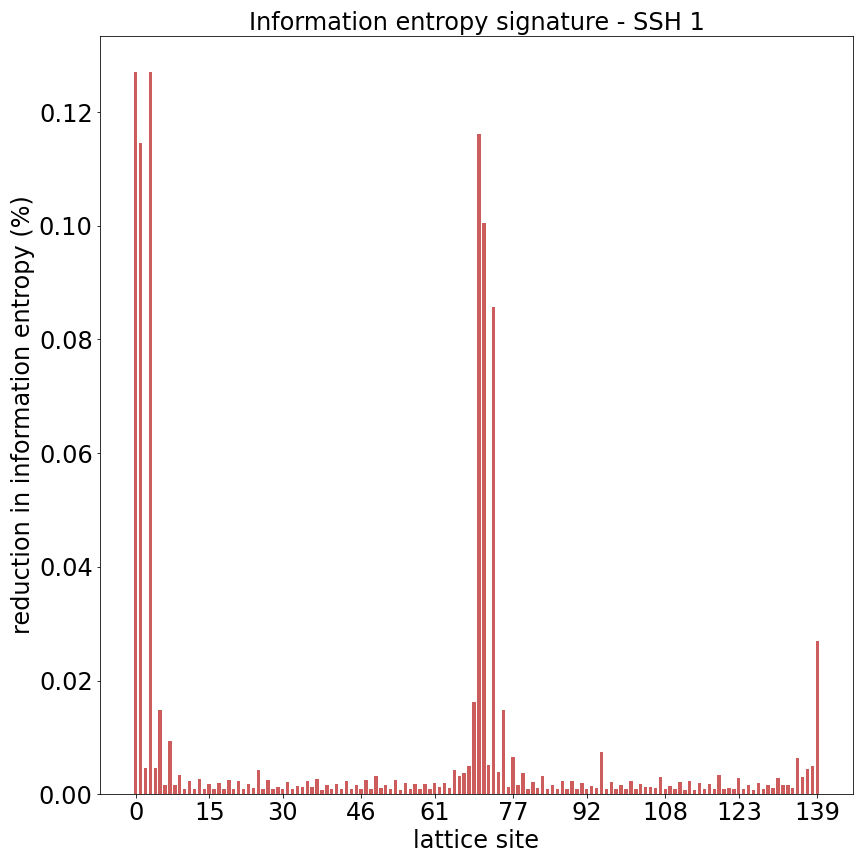
\includegraphics[width=.32\textwidth]{./supp_figures/ssh1/periodic_140_6561/plot_feature_importances.png}}
\subfigure[]{\label{feature_importances_ssh1_180}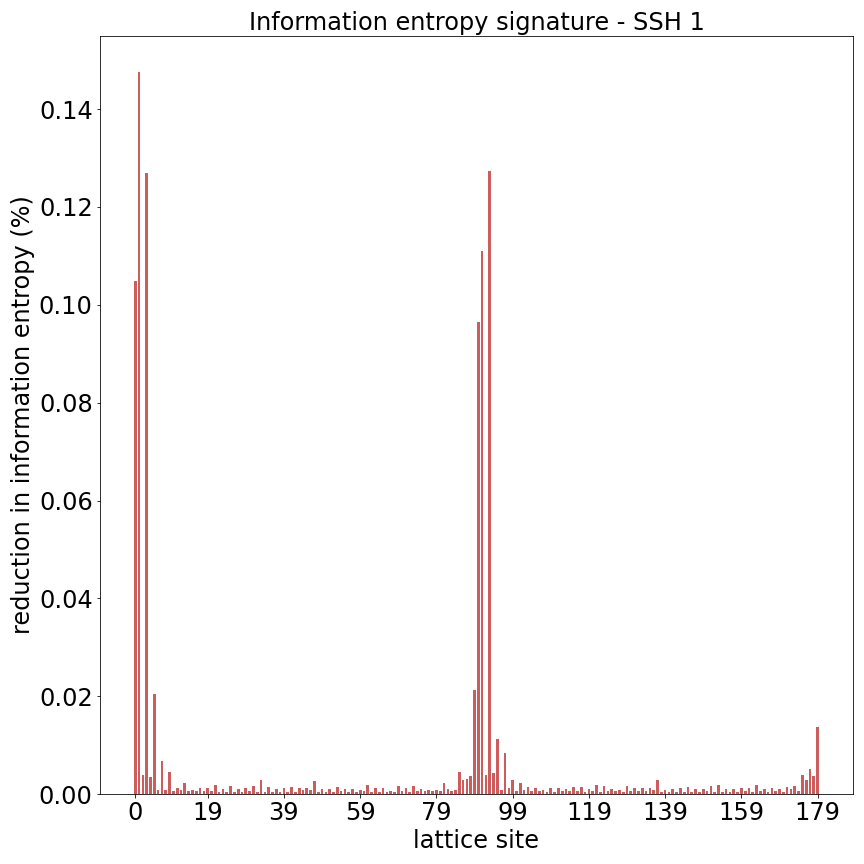
\includegraphics[width=.32\textwidth]{./supp_figures/ssh1/periodic_180_6561/plot_feature_importances.png}}
\subfigure[]{\label{feature_importances_ssh1_220}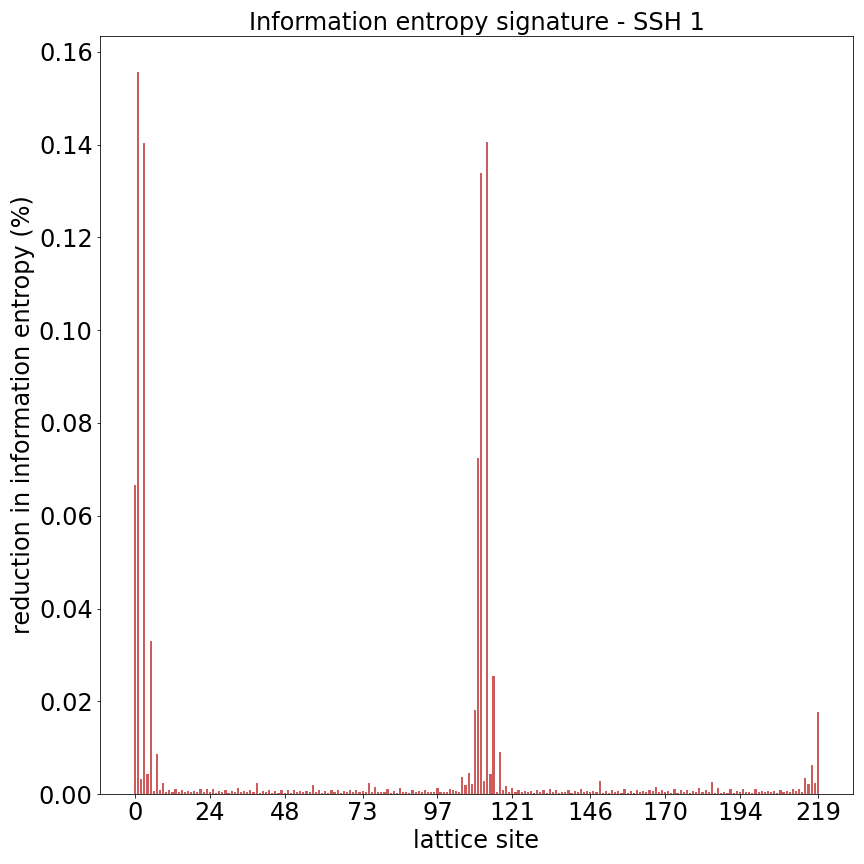
\includegraphics[width=.32\textwidth]{./supp_figures/ssh1/periodic_220_6561/plot_feature_importances.png}}
\caption{Information entropy signatures obtained for experiment 1 with higher lattice sizes. (a) Information entropy signature for 70 unit cells. (b) Information entropy signature for 90 unit cells. (c) Information entropy signature for 110 unit cells.}
\label{feature_importances_ssh1_longer_lattices}
\end{figure}
\begin{figure}
\centering
\subfigure[]{\label{feature_importances_ssh2_140}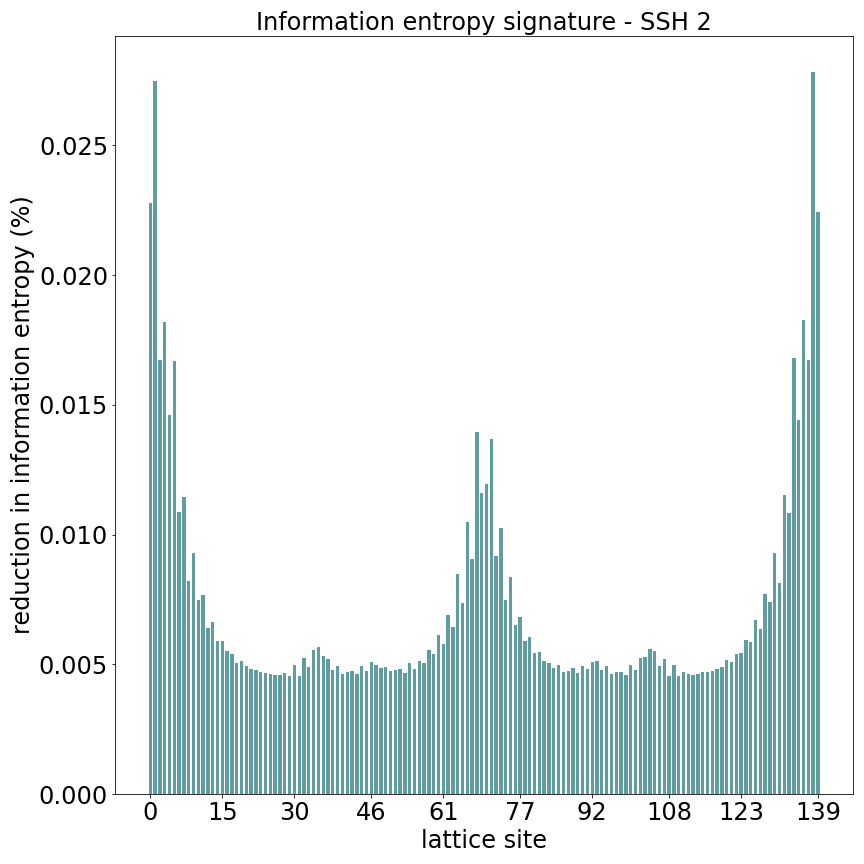
\includegraphics[width=.32\textwidth]{./supp_figures/ssh2/periodic_140_6561/plot_feature_importances.png}}
\subfigure[]{\label{feature_importances_ssh2_180}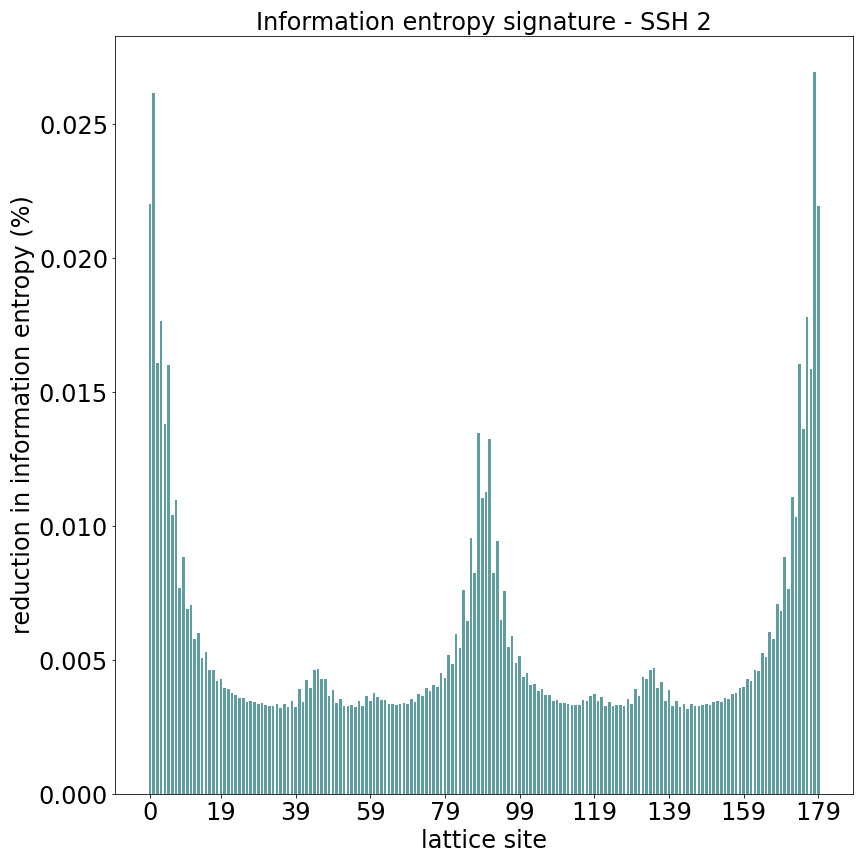
\includegraphics[width=.32\textwidth]{./supp_figures/ssh2/periodic_180_6561/plot_feature_importances.png}}
\subfigure[]{\label{feature_importances_ssh2_220}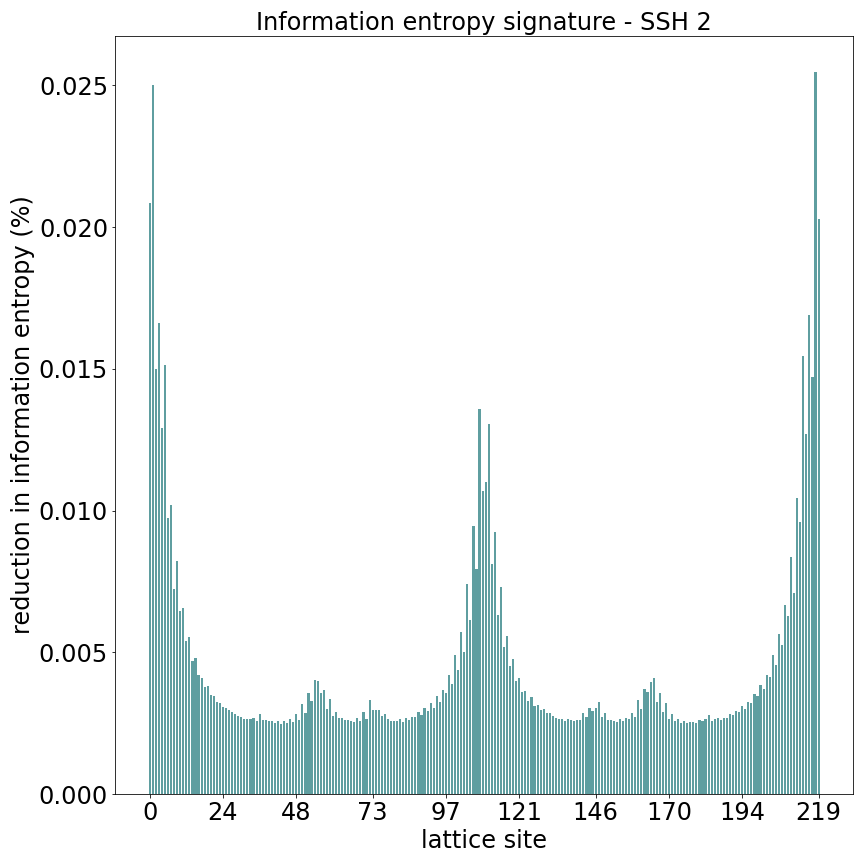
\includegraphics[width=.32\textwidth]{./supp_figures/ssh2/periodic_220_6561/plot_feature_importances.png}}
\caption{Information entropy signatures obtained for experiment 2 with higher lattice sizes. (a) Information entropy signature for 70 unit cells. (b) Information entropy signature for 90 unit cells. (c) Information entropy signature for 110 unit cells.}
\label{feature_importances_ssh2_longer_lattices}
\end{figure}

\begin{figure}
\centering
\subfigure[]{\label{cumulative_entropy_ssh1_140}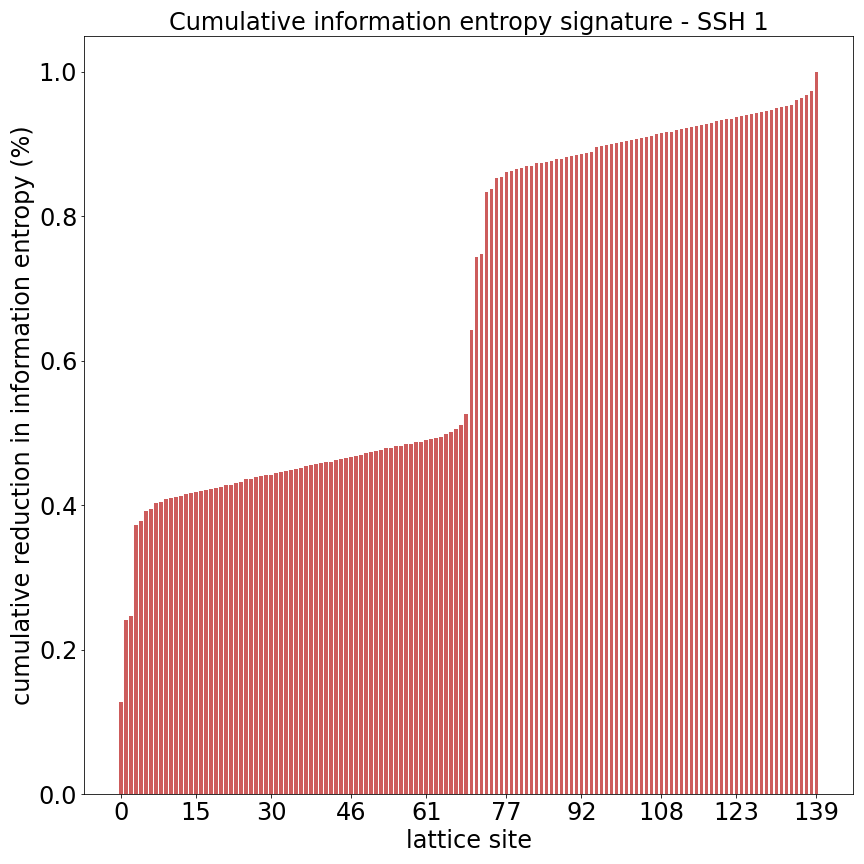
\includegraphics[width=.32\textwidth]{./supp_figures/ssh1/periodic_140_6561/plot_cumulative_feature_importances}}
\subfigure[]{\label{cumulative_entropy_ssh1_180}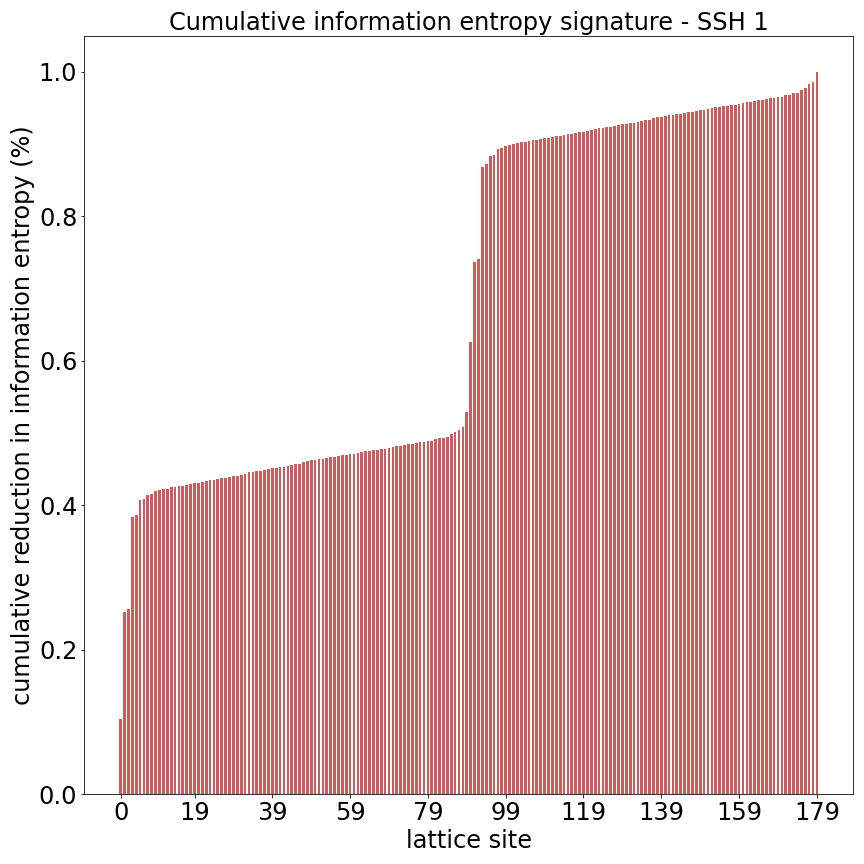
\includegraphics[width=.32\textwidth]{./supp_figures/ssh1/periodic_180_6561/plot_cumulative_feature_importances}}
\subfigure[]{\label{cumulative_entropy_ssh1_220}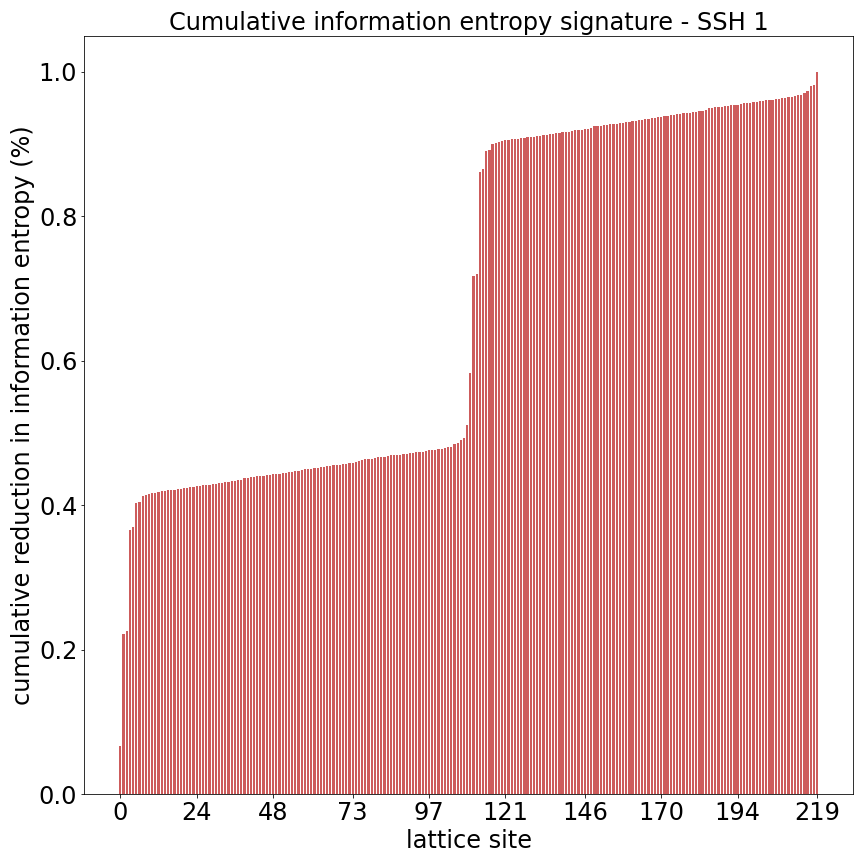
\includegraphics[width=.32\textwidth]{./supp_figures/ssh1/periodic_220_6561/plot_cumulative_feature_importances}}
\caption{Cumulative entropy distributions for higher lattice sizes in experiment 1. (a) Cumulative entropy distribution for 70 unit cells. (b) Cumulative entropy distribution for 90 unit cells. (c) Cumulative entropy distribution for 110 unit cells.}
\label{cdf1}
\end{figure}

\begin{figure}
\centering
\subfigure[]{\label{cumulative_entropy_ssh2_140}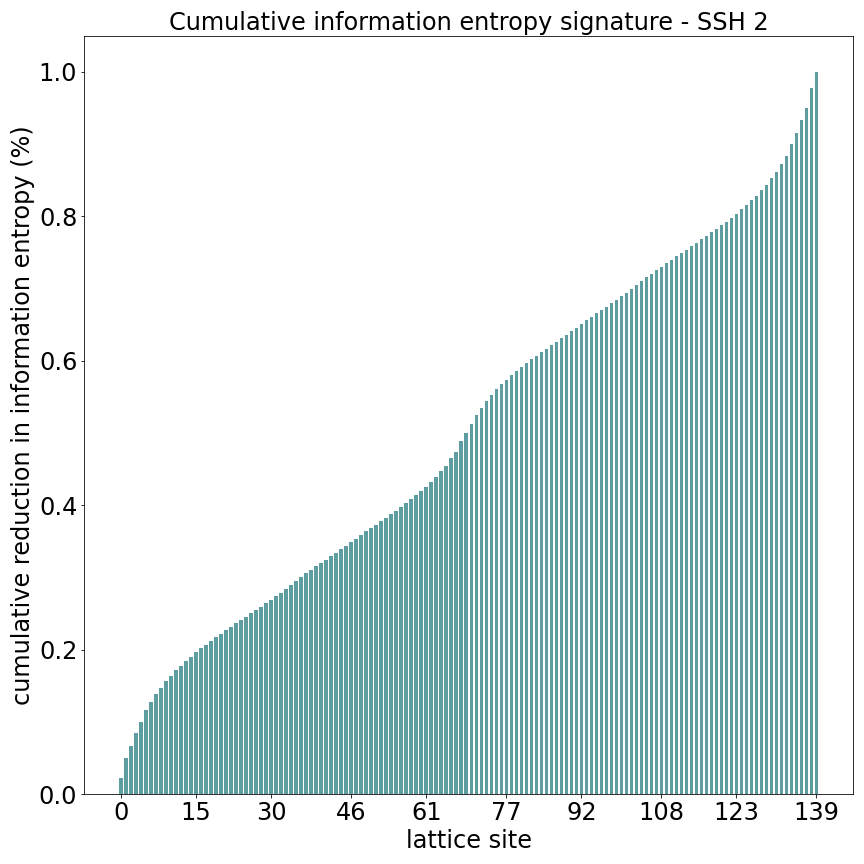
\includegraphics[width=.32\textwidth]{./supp_figures/ssh2/periodic_140_6561/plot_cumulative_feature_importances}}
\subfigure[]{\label{cumulative_entropy_ssh2_180}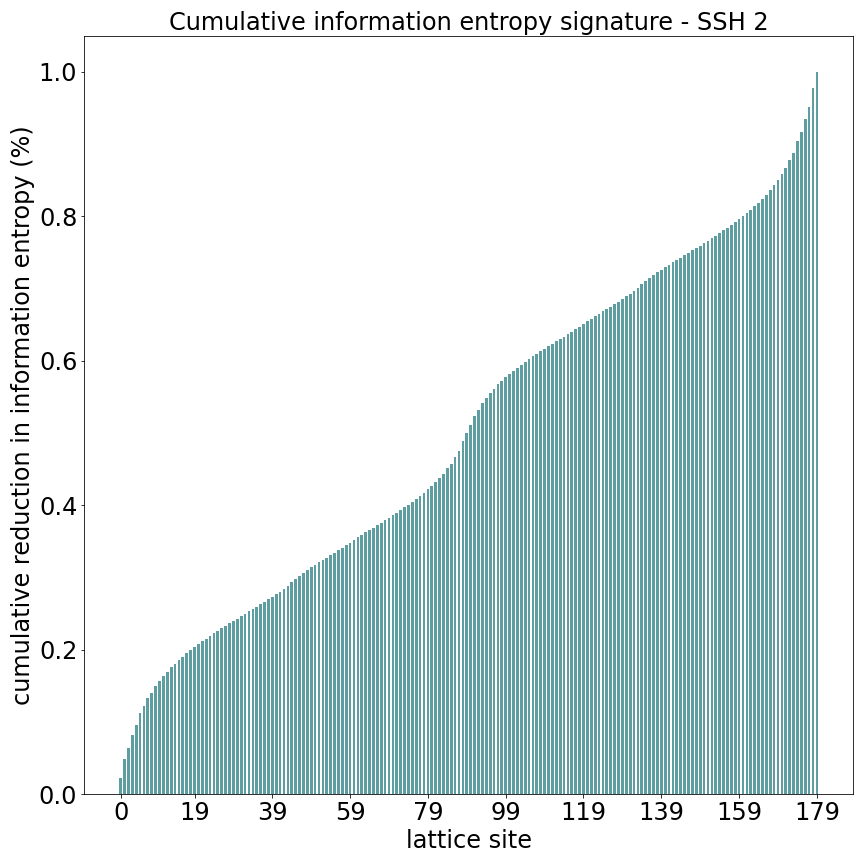
\includegraphics[width=.32\textwidth]{./supp_figures/ssh2/periodic_180_6561/plot_cumulative_feature_importances}}
\subfigure[]{\label{cumulative_entropy_ssh2_220}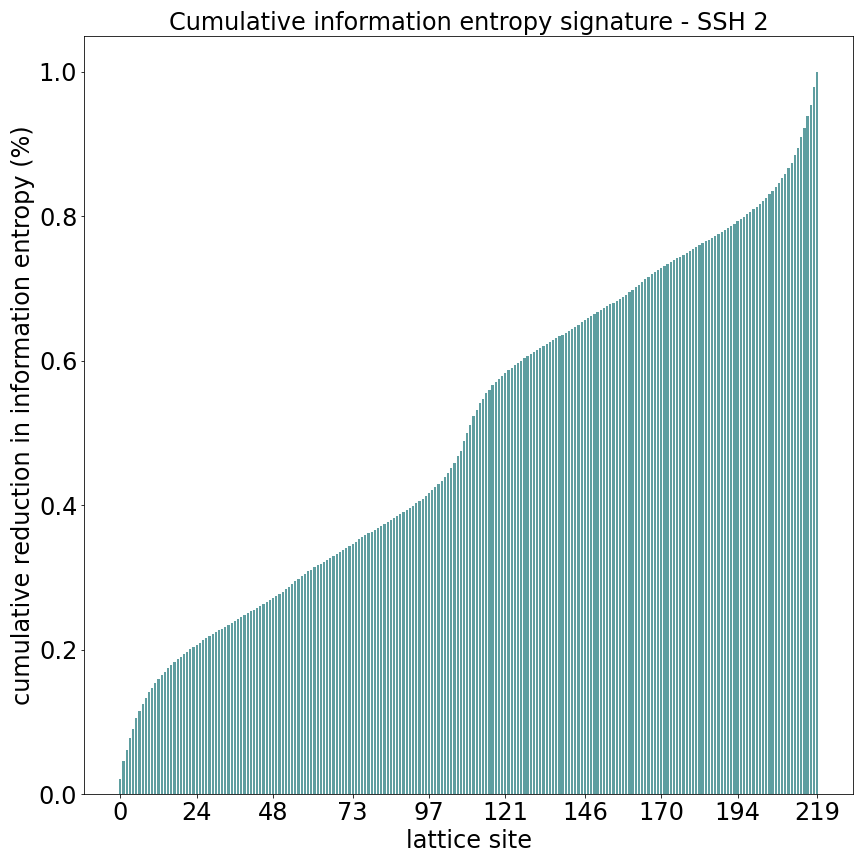
\includegraphics[width=.32\textwidth]{./supp_figures/ssh2/periodic_220_6561/plot_cumulative_feature_importances}}
\caption{Cumulative entropy distributions for higher lattice sizes in experiment 2. (a) Cumulative entropy distributions for 70 unit cells. (b) Cumulative entropy distributions for 90 unit cells. (c) Cumulative entropy distributions for 110 unit cells.}
\label{cdf2}
\end{figure}

%\newpage
%\bibliographystylesupp{ieeetr}
%\bibliographysupp{supp}

\begin{thebibliography}{10}
\bibitem{asboth2016short}
J.~K. Asb{\'o}th, L.~Oroszl{\'a}ny, and A.~P{\'a}lyi, ``A short course on
  topological insulators,'' {\em Lecture notes in physics}, vol.~919, 2016.

\bibitem{goodfellow2016deep}
I.~Goodfellow, Y.~Bengio, and A.~Courville, {\em Deep learning}.
\newblock MIT press, Cambridge, MA, USA, 2016.

\bibitem{bishop2006pattern}
C.~M. Bishop, {\em Pattern recognition and machine learning}.
\newblock Springer New York, NY, USA, 2006.

\bibitem{cayton2005algorithms}
L.~Cayton, ``Algorithms for manifold learning,'' {\em Univ. of California at
  San Diego Tech. Rep}, vol.~12, no.~1-17, p.~1, 2005.

\bibitem{narayanan2010sample}
H.~Narayanan and S.~Mitter, ``Sample complexity of testing the manifold
  hypothesis,'' in {\em Advances in Neural Information Processing Systems},
  pp.~1786--1794, 2010.

\bibitem{rifai2011manifold}
S.~Rifai, Y.~N. Dauphin, P.~Vincent, Y.~Bengio, and X.~Muller, ``The manifold
  tangent classifier,'' in {\em Advances in Neural Information Processing
  Systems}, pp.~2294--2302, 2011.
\end{thebibliography}



\end{document}
